\documentclass[reqno]{amsart}
\usepackage[utf8]{inputenc}
\usepackage[margin=1in]{geometry}
\usepackage[usenames, dvipsnames]{xcolor}
\usepackage{graphicx}
\usepackage{mathtools}
\usepackage{amssymb}
\usepackage{amsthm}
\usepackage{fancyhdr}
\usepackage{adforn}
\usepackage{xparse}
\usepackage{tikz}
\usetikzlibrary{fadings}
%\usetikzlibrary{matrix, positioning, calc}
% Additional math macros that I want in both my notes and my psets
\usepackage[sc, noBBpl]{mathpazo}
\usepackage{mathrsfs}
\usepackage[T1]{fontenc}
\usepackage{calligra}
\usepackage{microtype}
\usepackage[all]{xy}
\usepackage{slashed}
\newcommand{\A}{\mathbb A}
\newcommand{\cat}{\mathsf}
\newcommand{\sC}{\cat C}
\newcommand{\sD}{\cat D}
\newcommand{\sS}{\cat S}
\newcommand{\sA}{\mathscr A}
\newcommand{\sF}{\mathscr F}
\newcommand{\sG}{\mathscr G}
\renewcommand{\P}{\mathbb P}
\newcommand{\cO}{\mathscr O}
\newcommand{\sI}{\mathscr I}
\DeclareMathOperator{\coker}{coker}
\renewcommand{\Im}{\operatorname{Im}}
\newcommand{\pt}{\mathrm{pt}}
\DeclareMathOperator{\Hom}{Hom}
\newcommand{\op}{^{\mathsf{op}}}
\newcommand{\Id}{\mathrm{Id}}
\DeclareMathOperator{\Mat}{Mat}
\newcommand{\m}{\mathfrak m}
%\newcommand{\p}{\mathfrak p}
\newcommand{\q}{\mathfrak q}
\DeclareMathOperator{\MSpec}{MSpec}
\DeclareMathOperator{\Spec}{Spec}
\newcommand{\Top}{\cat{Top}}
\newcommand{\Ring}{\cat{Ring}}
\newcommand{\Mod}{\cat{Mod}}
\DeclareMathOperator{\res}{res}
\newcommand{\Alg}{\cat{Alg}}
\newcommand{\Fun}{\cat{Fun}}
\newcommand{\AffSch}{\cat{AffSch}}
\newcommand{\Ab}{\cat{Ab}}
\DeclareMathOperator{\bl}{--}
\DeclareMathOperator{\Free}{Free}
\DeclareMathOperator{\For}{For}
\newcommand{\Set}{\cat{Set}}
\newcommand{\LocRing}{\cat{LocRing}}
\newcommand{\Grp}{\cat{Grp}}
\newcommand{\Sch}{\cat{Sch}}
\newcommand{\inHom}{\operatorname{\underline{\Hom}}}
\DeclareMathOperator{\Frac}{Frac}
\DeclareMathOperator{\Gal}{Gal}
\DeclareMathOperator{\Nil}{Nil}
\newcommand{\pre}{\sC^{\text{pre}}}
\newcommand{\sh}{_{\text{sh}}}
\newcommand{\G}{\mathbb G}
\DeclareMathOperator{\Proj}{Proj}
\newcommand{\sM}{\mathscr M}
\newcommand{\sV}{\mathscr V}
\newcommand{\fU}{\mathfrak U}
\newcommand{\GL}{\mathrm{GL}}
\DeclareMathOperator{\Sym}{Sym}
% http://tex.stackexchange.com/questions/141434/how-to-type-sheaf-hom
\DeclareMathOperator{\shom}{\mathscr{H}\text{\kern -4pt {\calligra\large om}}\,}
\newcommand{\sL}{\mathscr L}
\DeclareMathOperator{\QC}{QC}
\DeclareMathOperator{\Supp}{Supp}
\newcommand{\sN}{\mathscr N}
\DeclareMathOperator{\Ann}{Ann}
\DeclareMathOperator{\Der}{Der}
\newcommand{\ctcpx}[1]{(#1)^{\text{der}}}
\newcommand{\Dist}{\mathsf{Dist}}
\newcommand{\shdi}{\operatorname{Sh}_{\Dist}}
\DeclareMathOperator{\Sh}{Sh}
\newcommand{\shz}{\mathsf{Sh}_{\text{\rm Zar}}}
\DeclareMathOperator{\Gr}{Gr}
% Source: http://tug.org/pipermail/xy-pic/2001-July/000015.html
\newcommand{\pullbackcorner}[1][dr]{\save*!/#1+1.2pc/#1:(1,-1)@^{|-}\restore}
\newcommand{\pushoutcorner}[1][dr]{\save*!/#1-1.2pc/#1:(-1,1)@^{|-}\restore}
\newcommand{\TDel}{\mathrm{2\Delta}}
\DeclareMathOperator{\Bl}{B\ell}
\newcommand{\cR}{\mathcal R}
\newcommand{\cL}{\mathcal L}
\newcommand{\cH}{\mathcal H}
\newcommand{\refR}{\reflectbox{\(\cR\)}}

\renewcommand{\a}{\alpha}
\renewcommand{\b}{\beta}
%\newcommand{\e}{\epsilon}
\renewcommand{\l}{\lambda}
\renewcommand{\L}{\Lambda}
\newcommand{\g}{\gamma}
\newcommand{\s}{\sigma}
\newcommand{\z}{\zeta}
\newcommand{\RR}{\mathbb{R}}
\newcommand{\NN}{\mathbb{N}}
\newcommand{\QQ}{\mathbb{Q}}
\newcommand{\ZZ}{\mathbb{Z}}
\newcommand{\CC}{\mathbb{C}}
\newcommand{\cC}{\mathcal{C}}
\newcommand{\f}{\frac}
\newcommand{\p}{\partial}
\renewcommand{\P}[3][]{\f{\partial^{#1} #2}{\partial #3 ^{#1}}}
%\newcommand{\avg}[1]{\langle #1 \rangle}
\newcommand{\avg}[1]{\left< #1 \right>}
\newcommand{\?}{\overset{?}{=}}
\newcommand{\Int}{\int_{-\infty}^\infty}
\newcommand{\ket}[1]{\left| #1 \right>} % for Dirac bras
\newcommand{\bra}[1]{\left< #1 \right|} % for Dirac kets
\newcommand{\braket}[2]{\left< #1 \vphantom{#2} \right|
 \left. #2 \vphantom{#1} \right>} % for Dirac brackets
\newcommand{\pv}{\vec{p}}

\newcommand{\grad}[1]{\gv{\nabla} #1} % for gradient
\let\divsymb=\div % rename builtin command \div to \divsymb
\renewcommand{\div}[1]{\gv{\nabla} \cdot #1} % for divergence
\newcommand{\curl}[1]{\gv{\nabla} \times #1} % for curl
\renewcommand{\labelenumi}{(\alph{enumi})}
\let\vaccent=\v % rename builtin command \v{} to \vaccent{}
\renewcommand{\v}[1]{\ensuremath{\mathbf{#1}}}
\newcommand{\uv}[1]{\ensuremath{\mathbf{\hat{#1}}}} % for unit vector
\newcommand{\gv}[1]{\ensuremath{\mbox{\boldmath$ #1 $}}} 
% for vectors of Greek letters
\usepackage{hyperref}
\usepackage{siunitx}

%\usepackage[compat=1.1.0]{tikz-feynman}

% TODO fiddle with colors
\definecolor{newblue}{HTML}{1F98A6}
\definecolor{newred}{HTML}{D95448}
\definecolor{neworange}{HTML}{F29441}
\hypersetup{
	colorlinks,
	linkcolor=newred,
	citecolor=neworange,
	urlcolor=newblue!80!black,
}
\usepackage[all]{hypcap}
\pagestyle{plain}
\setcounter{tocdepth}{1}


\usepackage{titlesec}
\titleformat{\section}[frame]
  {\normalfont}
  {\filright
   \footnotesize
   \enspace Lecture \arabic{section}.\enspace}
  {8pt}
  {\Large\bfseries\filcenter}
\usepackage[dotinlabels]{titletoc}
\titlecontents{section}[1.5em]{}{\contentslabel{2.3em}}{\hspace*{-2.3em}}{\hfill\contentspage}

\renewcommand{\sectionmark}[1]{\markleft\thesection. #1}

\fancyhf{}
\fancyhead[RO,LE]{\small\thepage}
\fancyhead[LO]{\small\slshape\nouppercase{\rightmark}}
\fancyhead[RE]{\small\slshape Advanced Quantum Field Theory Lecture Notes}
\setlength{\headheight}{11.0pt}
\pagestyle{fancy}

\numberwithin{equation}{section}
\newcommand{\orbreak}{
\begin{center}
	\adforn{17}\;\(\cdot\)\;\adforn{18}
	\vspace{0.2cm}
\end{center}
}

\renewcommand{\labelitemi}{\(\circ\)}

% I wanted to allow one to reference parts of a thm/cor/etc. and have it print the thm number too, e.g. 29.2(1),
% but this isn't working right now. Probably the best way to do this would be to play around with enumitem to
% define a new enumerate-like counter and then just use that directly instead of enumerate in comp.

% This feels really wobbly, but so far it's working
\NewDocumentEnvironment{comp}{mm}{%
	\csname #1\endcsname\hfill
	\csname #2\endcsname
}{
	\csname end#2\endcsname
	\csname end#1\endcsname
}

% usage:
% \shortexact[f][g]{A}{B}{C},
%
%			 f    g
% for 0 -> A -> B -> C -> 0,
\DeclareDocumentCommand{\shortexact}{O{} O{} mmmm}{
\xymatrix{
	0\ar[r] & #3\ar[r]^-{#1} & #4\ar[r]^-{#2} & #5\ar[r] & 0#6
}}
% exactly the same, but for 0 -> A -> B -> C
\DeclareDocumentCommand{\leftexact}{O{} O{} mmmm}{
\xymatrix{
	0\ar[r] & #3\ar[r]^-{#1} & #4\ar[r]^-{#2} & #5 #6
}}
% ... and the same, for A -> B -> C -> 0
\DeclareDocumentCommand{\rightexact}{O{} O{} mmmm}{
\xymatrix{
	#3\ar[r]^-{#1} & #4\ar[r]^-{#2} & #5\ar[r] & 0#6
}}



% usage:
% X\dblarrow[r] & Y
%   f
% X => Y
%   g
\DeclareDocumentCommand{\dblarrow}{O{} O{} O{}}{
	\ar@<0.4ex>[#1]^-{#2}\ar@<-0.4ex>[#1]_-{#3}
}
% Note: it would be a useful exercise to figure out how to define this so it can be used as
% \dblarrow[r]^f_g

\everyentry={\displaystyle}

\newcommand{\N}{\mathbb N}
\newcommand{\Z}{\mathbb Z}
\newcommand{\Q}{\mathbb Q}
\newcommand{\R}{\mathbb R}
\newcommand{\C}{\mathbb C}
\newcommand{\F}{\mathbb F}
\newcommand{\vp}{\varphi}
\newcommand{\term}{\emph}
\renewcommand{\vec}[1]{\boldsymbol{\mathbf{#1}}}
\DeclarePairedDelimiter\paren{(}{)}
%\DeclarePairedDelimiter\ang{\langle}{\rangle}
\DeclarePairedDelimiter\abs{\lvert}{\rvert}
\DeclarePairedDelimiter\norm{\lVert}{\rVert}
\DeclarePairedDelimiter\bkt{[}{]}
\DeclarePairedDelimiter\set{\{}{\}}
% Swap paren* and paren, etc., so that the normal version resizes by default.
% Meanwhile, one can use \paren*[\Big]{...} to customize the size easily.
% It would be interesting to wrap this up into a custom \definedelimiter command...
\makeatletter
	\let\oldparen\paren
	\def\paren{\@ifstar{\oldparen}{\oldparen*}}
	\let\oldbkt\bkt
	\def\bkt{\@ifstar{\oldbkt}{\oldbkt*}}
\makeatother
\newcommand{\e}{\varepsilon}
\def\qedsymbol{{\small{\ensuremath{\boxtimes}}}}
\newcommand{\inj}{\hookrightarrow}
\newcommand{\surj}{\twoheadrightarrow}
\DeclareMathOperator{\id}{id}
\newcommand{\ud}{\,\mathrm{d}}
\renewcommand{\d}{\mathrm d}
\newcommand{\dfr}[2]{\frac{\mathrm d #1}{\mathrm d #2}}
\newcommand{\pfr}[2]{\frac{\partial #1}{\partial #2}}

%\catcode`\"=13
%\newcommand{"}[1]{^{(#1)}}
\newtheorem{thm}[equation]{Theorem}
\newtheorem*{thm*}{Theorem}
\newtheorem{lem}[equation]{Lemma}
\newtheorem*{lem*}{Lemma}
\newtheorem{cor}[equation]{Corollary}
\newtheorem{prop}[equation]{Proposition}
\newtheorem{obs}[equation]{Observation}
\theoremstyle{definition}
\newtheorem{ex}[equation]{Exercise}
\newtheorem{exm}[equation]{Example}
\newtheorem{defn}[equation]{Definition}
\newtheorem*{claim}{Claim}
\theoremstyle{remark}
\newtheorem*{rem}{Remark}
\newtheorem*{fct}{Fact}
\newtheorem*{note}{Note}

\begin{document}
\title{General Relativity}
\author{Ian Lim\\ Michaelmas 2018}
\maketitle
{\small\noindent These notes were taken for the \textit{General Relativity} course taught by Malcolm Perry at the University of Cambridge as part of the Mathematical Tripos Part III in Michaelmas Term 2018. I live-\TeX ed them using TeXworks, and as such there may be typos; please send questions, comments, complaints, and corrections to 
\href{mailto:itel2@cam.ac.uk?subject=GR\%20Lecture\%20Notes}{\texttt{itel2@cam.ac.uk}}.\\
Many thanks to Arun Debray for the {\LaTeX} template for these lecture notes: as of the time of writing, you can find him at \url{https://web.ma.utexas.edu/users/a.debray/}.}

\tableofcontents

\section{Friday, October 5, 2018}
	Unlike in previous years, this course is intended to be a stand-alone course on general relativity, building up the mathematical formalism needed to construct the full theory and explore some examples of interesting spacetime metrics. It is linked to the Black Holes course taught in Lent term, which I will also be writing notes for.

Some recommended course materials and readings include the following:
\begin{itemize}
\item Sean Carroll, Spacetime and Geometry
\item Misner, Thorne, and Wheeler, Gravitation
\item Wald, General Relativity
\item Zee, Einstein Gravity in a Nutshell
\item Hawking and Ellis, ``The Large Scale Structure of Spacetime''
\end{itemize}

In Minkowski\footnote{I've heard some USAmericans pronounce this ``min-cow-ski.'' In German, it is ``min-koff-ski.''} spacetime (flat space) we specify points in spacetime by spatial coordinates in $\RR^3$, i.e. the Cartesian coordinates $(x,y,z)$, plus a time coordinate $t$. The line element (spacetime separation) is given by the metric
$$ds^2=-dt^2+dx^2+dy^2+dz^2.$$
$ds$ is the proper distance between $x$ and $x+dx$, $y$ and $y+dy$, $z$ and $z+dz$, and $t$ and $t+dt$. (As is typical in relativity, we work in units where $c=1$. Note that the metric sign convention here is flipped from my QFT notes, which uses the ``mostly minus'' convention-- this is arbitrary and so long as one is consistent it makes no difference.) Using the Einstein summation convention, the metric is usually written more compactly as $$ds^2=\eta_{\alpha\beta}x^\alpha x^\beta,$$ with $\eta_{\alpha\beta}$ the Minkowski space metric.

Let's recall from special relativity that we call separations with $ds^2>0$ ``spacelike,'' with $ds^2<0$ ``timelike,'' and $ds^2=0$ null (or occasionally lightlike).
\begin{defn}
The \term{chronological future} of a point $p$ is the set of all points that can be reached from $p$ along future directed timelike lines, and we call this $I^+(p)$. It is the interior of the future-directed light cone. Conversely we have the chronological past of $p$, $I^-(p)$, which is the interior of the past-directed light cone. We also have the \term{causal future} of $p$, which is the set of all points that can be reached from $p$ along future-directed timelike \emph{or} null lines, and we call this $J^+(p)$. Similarly we have the causal past, $J^-(p)$. Thus $J$ is the closure of $I$ and is the interior \emph{plus} the light cone itself.
\end{defn}

\begin{figure}
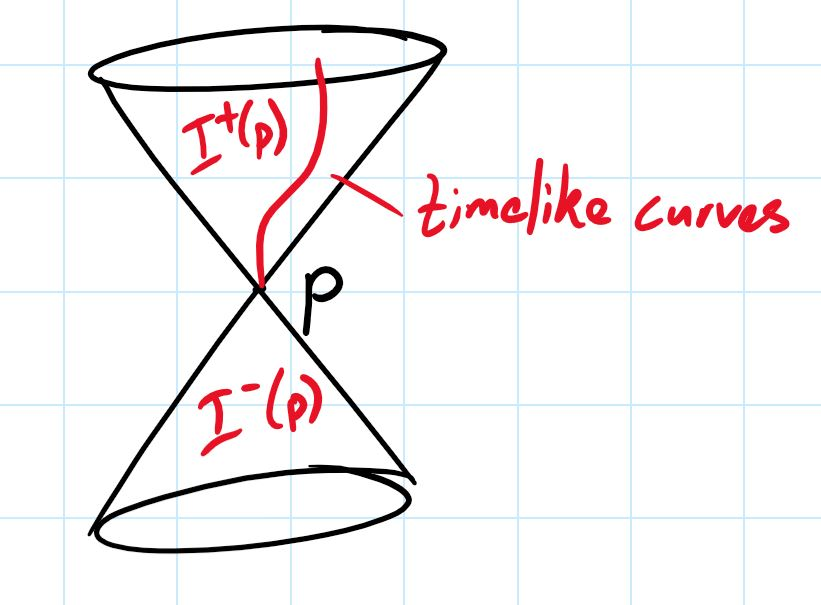
\includegraphics{2018/10/20181005_img1}
\caption{An illustration of the light cones from a point $p$, plus the chronological future $I^+$ and chronological past $I^-$. Also depicted in red is a timelike curve (e.g. a possible particle trajectory in spacetime).}
\end{figure}

Let $x^a(\tau)$ be a curve in spacetime.\footnote{Evidently we are not using the convention that Greek indices range from $0$ to $3$ and Latin indices range from $1$ to $3$. I have copied the lecturer's convention here, but may change to more traditional notation if it becomes relevant.} Then the tangent vector to the curve is $u^a=\frac{dx^a}{d\tau}$. For timelike curves, $u^a u^b \eta_{ab}=-1 \iff \tau$ is the proper time along the curve.
\footnote{The property that $U^\alpha U^\beta \eta_{\alpha\beta}=-1$ is easy to prove. See the Special Relativity catch-up sheet found \href{http://www.maths.cam.ac.uk/sites/www.maths.cam.ac.uk/files/grspecialrelativity.pdf}{here} for some nice exercises in SR: this is exercise 3. Assuming the result of exercise 2 which states that the four-velocity of a massive particle is $U^\mu=\gamma(1,v^i)$, we then have $U\cdot U =\gamma^2(-1+v^2)=\frac{v^2-1}{1-v^2}=-1$. Since this is a fully contracted expression (no indices floating around), it is true in all frames.}
We also know that $\int_p^q d\tau = \Delta \tau$, which just says that the integral of $d\tau$ along a curve from $p$ to $q$ yields the proper time interval, what a clock actually measures.

We also remark that Minkowski space has some very nice symmetries. Since $x,y,$ and $z$ do not appear explicitly in the metric, our spacetime is invariant under translations. It is also invariant under rotations in $\RR^3$. It would be nice to extend rotations to include the time coordinate $t$ as well-- this is exactly what a Lorentz transformation does.

Lorentz transformations in general involve time-- they are defined by the matrices $\Lambda$ which satisfy
$$\Lambda^T \eta \Lambda= \eta,$$
i.e. they preserve the inner product $\eta$ in Minkowski space, forming the group $O(3,1)$. Lorentz transformations consist of rotations in $\RR^3$ and boosts. This is equivalent to the defining property of rotation matrices $R$ that $R^T \delta R=\delta$, meaning that rotation matrices preserve the standard Euclidean inner product in $\RR^3$ and form the group $O(3)$.\footnote{Strictly, $O(3)$ also includes reflections-- for matrices which preserve both orientation and the inner product, we must also require that $\det R=+1$, defining the group $SO(3)$. We'll see a similar caveat with the Lorentz group in just a second.}
Written explicitly, the Lorentz boost in the $x$-direction to a frame moving with velocity $v$ is
\begin{eqnarray*}
t\to t'&=&\frac{t-vx}{\sqrt{1-v^2}}\\
x\to x'&=&\frac{x-vt}{\sqrt{1-v^2}}\\
y\to y'&=&y\\
z\to z'&=&z
\end{eqnarray*}
We may also write it in matrix notation,
$${\Lambda^a}_b =
\begin{pmatrix}
\gamma&-\gamma v &0 & 0\\
-\gamma v & \gamma & 0 & 0\\
0&0&1&0\\
0&0&0&1
\end{pmatrix}$$
where $\gamma$ is defined in the usual way by $\gamma \equiv \frac{1}{\sqrt{1-v^2}}$.

Rather than constructing the (in general complicated) Lorentz boost in an arbitrary direction, it is often more convenient to rotate one's frame of reference in $\RR^3$ so the boost is in the new $x$-direction, perform the Lorentz boost, and then transform back:
$$R^T \Lambda R= \Lambda_R,$$
where $\Lambda_R$ is a new Lorentz transformation.\footnote{It's easy to check that $\Lambda_R$ really is a Lorentz transformation-- just observe that rotations alone are a subset of Lorentz transformations, since they preserve the inner product on $\RR^3$ and do not affect the time coordinate. In the language of group theory, rotations form an $SO(3)$ subgroup of the full Lorentz group $O(3,1)$-- see Definition \ref{lorentzgroup}. Therefore any combination of rotations and Lorentz boosts will form another valid Lorentz transformation by the group closure property.}

\begin{defn}\label{lorentzgroup}
The Lorentz transformations taken together form the \term{Lorentz group}. It satisfies the group axioms of identity, unique inverses (since $\det\Lambda \neq 0$), associativity (from associativity of matrix multiplication), and closure (see footnote for proof).\footnote{More precisely, we know that the determinant is nonzero since $-1=\det{\eta}=\det(\Lambda^T\eta\Lambda)=\det(\Lambda^T)\det(\eta)\det(\Lambda)=(-1)\det(\Lambda)^2\implies \det(\Lambda)=\pm 1 \neq 0$. To prove closure, suppose $\Lambda_1,\Lambda_2$ are Lorentz transformations. The product $\Lambda_1\Lambda_2$ then satisfies $(\Lambda_1\Lambda_2)^T \eta(\Lambda_1\Lambda_2)= \Lambda_2^T \Lambda_1^T \eta\Lambda_1 \Lambda_2 = \Lambda_2^T \eta \Lambda_2 = \eta$, so $\Lambda_1\Lambda_2$ is also a Lorentz transformation.}
\end{defn}

$\Lambda$ can include reflections in time or space. To avoid such complications, we sometimes refer to the \term{proper orthochronous Lorentz group,} i.e. to exclude space and time reversals, but often we are more careless and simply call it the Lorentz group.
\begin{defn}
The \term{Poincar\'e group} is then the semidirect product of Lorentz transformations and translations. This is the group of symmetries of Minkowski space.
\end{defn}
We have translations defined as
$$x^a\to {x^a}'=x^a+\Delta x^a$$
and also Lorentz transformations, with the property
$${(\Lambda^T)_a}^c \eta_{cd} {\Lambda^d}_b=\eta_{ab}.$$


\begin{defn}
We also have \term{contravariant vectors} (indices up) written $u^a$ and their corresponding \term{covariant} vectors (indices down) $$u_a\equiv\eta_{ab}u^b,$$ where we have used the metric to lower an index. These are sometimes equivalently called simply vectors and covectors. We can also raise indices using the inverse metric $\eta^{ab}$ (defined by $\eta^{ab}\eta_{bc}=\delta^a_c$). Thus
$$u^b=\eta^{ba}u_a.$$
\end{defn}

We define the Lorentz transformation of a contravariant vector as
$u^a\to {u^a}' = {\Lambda^a}_b u^b.$  For instance, $x^a$ is an example of a contravariant vector.

\begin{defn}
A \term{scalar} is an object which is invariant under a Lorentz transformation. We saw that a covariant vector transforms with right multiplication by the Lorentz transformation, whereas a contravariant vector transforms by left multiplication. 

More generally, a \term{tensor of type $(r,s)$} transforms with $r$ copies of the Lorentz transformation on the $r$ up indices and $s$ copies of the Lorentz transformation on the $s$ down indices, 
\begin{equation}
{T^{\mu_1 \mu_2\ldots \mu_r}}_{\nu_1 \nu_2 \ldots \nu_s} \to {T^{\alpha_1 \alpha_2\ldots \alpha_r}}_{\beta_1 \beta_2 \ldots \beta_s}=\Lambda^{\alpha_1}_{\mu_1} \ldots \Lambda^{\alpha_r}_{\mu_r} {T^{\mu_1 \mu_2\ldots \mu_r}}_{\nu_1 \nu_2 \ldots \nu_s} \Lambda^{\nu_1}_{\beta_1}\ldots \Lambda^{\nu_s}_{\beta_s}
\end{equation}

By this definition, a scalar may be thought of as a type $(0,0)$ tensor, a contravariant vector a type $(1,0)$ tensor, and a covariant vector a type $(0,1)$ tensor.
\end{defn}

\section{Monday, October 8, 2018}
	Today, we'll start by remarking that Maxwell's equations can be written compactly in 4-vector format. Recall from a good course on electrodynamics that we define the electromagnetic field strength tensor $F^{\mu\nu}$ as
$$F^{\mu\nu}=\begin{pmatrix}
0& E_x & E_y & E_z\\
-E_x & 0 & B_z & - B_y\\
-E_y & -B_z & 0 & B_x\\
-E_z & B_y & -B_x & 0
\end{pmatrix}.$$
$F^{\mu\nu}$ is a totally antisymmetric rank two tensor. Defining the four-current $j^\mu \equiv(\rho, \vec{j})$ with $\vec{j}$ the ordinary current density and $\rho$ the charge density, we see that
$$\p_a F_{bc} +\p_b F_{ca} +\p_c F_{ab}=0$$
and
$$\p_a F^{ab}=-j^b.$$

But there's something strange about this-- these equations in their current form hold for Cartesian coordinates only. Of course, the laws of physics (as expressed through empirical results in experiments) cannot depend on the coordinate system we use to define them. 
\begin{exm}
The Minkowski metric takes the Cartesian form
$$ds^2=-dt^2+dx^2+dy^2+dz^2$$
but if we pass to spherical coordinates, the metric now takes the form 
$$ds^2=-dt^2+dr^2+r^2d\theta^2 +r^2 \sin^2 \theta d\phi^2=g_{ab}dx^a dx^b,$$
where $x^a=(t,r,\theta,\phi).$
\end{exm}

General relativity is thus motivated by a desire to understand how the laws of physics are invariant not just under Lorentz transformations but general coordinate transformations. It is also motivated by the \term{weak equivalence principle}, which states that inertial mass and gravitational mass are the same thing-- the $m$ in $F=ma$ and the $m$ in $F=-\frac{GMm }{r^2}$ are the same mass! This is closely related to the \term{Einstein equivalence principle}, which states that in a freely falling frame, the laws of physics are those of special relativity. One cannot distinguish between being in freefall under a gravitational field and simply being at rest in no gravitational field.

We consider spacetime to be a 4-dimensional system ($3+1$ dimensions, if you like) and in particular it has a manifold structure. We may make an explicit choice of some coordinates $\set{x^a}$ that label points in (a coordinate patch of) $M$, but it would be nice to define vectors in a way that is independent of the coordinates. This will lead us to revisit vectors and covectors.

Consider a parametrized curve $\lambda(\tau):\RR\to M$ sitting in $M$. Now take $f=f(x^a)$ to be a differentiable function of the coordinates, and define an operator that maps $f$ into the total derivative $df/dt$: by applying the chain rule, we have
$$\frac{df}{dt}=\P{x^a}{t}\left(\P{}{x^a}f\right).$$
Thus a vector $V$ is a linear differential operator that acts on $f$: explicitly, we can write $$V=\P{x^a}{t}\P{}{x^a},$$ where the $\P{x^a}{t}$ are called the components of the vector and denoted by $V^a$. The right way to think of a vector is as a coordinate-independent generalization of a directional derivative. The components will in general transform when we change coordinates, but the vector as an operator stays the same.

That said, a general vector can be written in its components in some coordinate basis $x^a$ as
$$V= V^a \P{}{x^a}.$$

Thinking back to our curve $\lambda(\tau)$, we may expand our coordinates locally as $x^a(\tau)=x^a (\tau_0)+V^a (\tau-\tau_0)+O((\tau-\tau_0)^2)$, where $V$ is the tangent vector to some curve through the point $\tau_0$. (Okay, we're being a bit careless with notation here-- the instructor has written $\lambda(t)$, but sometimes $t$ is a coordinate on the manifold.) Therefore we may also interpret (tangent) vectors as describing how our manifold curves locally about a point.

Vectors (as the name suggests) form a vector space.\footnote{We get most of the vector space axioms for free. Commutativity and associativity follow from doing component-wise addition in a basis, as does distributivity of scalar sums. The additive identity is the vector where all components are zero. The additive inverse for a vector with components $V^a$ is just $-V^a$. The scalar multiplication identity is automatic.} 
If $W, Y$ are vectors, $\alpha,\beta$ real numbers, then $\alpha W + \beta Y$ is another vector with components
$$(\alpha W^a+\beta Y^a)\P{}{x^a}.$$

As linear differential operators, vectors also obey the Leibniz rule
$$V^a \P{}{x^a}(fg)= V^a \P{f}{x^a} g+ f V^a \P{g}{x^a}.$$

The space of tangent vectors at a point $p$ is called $T_p(M)$. Recall that we defined our tangent vectors with respect to its components in some basis $x^a$. But if we now change to some new coordinates $\tilde x^b = \tilde x^b(x^a)$, then by the chain rule our basis vectors $\P{}{x^a}$ transform as
$$\P{}{x^a}=\P{\tilde x^{b}}{x^a}\frac{\partial}{\partial \tilde x^b}.$$
But $V$ as an operator is invariant-- it does not depend on our choice of coordinates, so its components must also change. If we rewrite $V$ in a different set of coordinates, we find that
$$V=V^a \P{}{x^a} = V^a \P{\tilde x^b}{x^a}\frac{\p}{\p\tilde x^b}$$
by the chain rule. Since $V$ is independent of basis,
$$V=V^a \P{}{x^a}= \tilde V^a \P{}{\tilde x^a},$$ so by comparison we see that the components of $V$ transform as
$$V^a\to \tilde V^{a'} = \frac{\p\tilde x^{a'}}{\p x^a} V^a.$$
In other words, tangent vectors transform as contravariant vectors, which we recognize as a generalization of the formula in special relativity where we had $$\P{\tilde x^{a'}}{x^a}=\Lambda^{a'}_{a}$$
with $\Lambda^{a'}_{a}$ the Lorentz transformation.

\begin{defn}
We may also define \term{one-forms}, which are covariant vectors at some point $p$. Thus the inner product $\langle \omega, V\rangle$ is a real number, with $\omega$ a 1-form and $V$ a vector. The inner product is bilinear:
if $V=\alpha Y + \beta W,$ then
$$\langle \omega, \alpha Y + \beta W\rangle = \alpha\langle \omega, Y\rangle +\beta \langle \omega, W\rangle$$
and similarly for the first argument, if $\omega = \alpha \eta+\beta \xi$
$$\ang{\alpha \eta +\beta\xi, V} = \alpha \ang{\eta, V} +\beta \ang{\xi, V}.$$
\end{defn}

Let us write $V$ in a basis, $V=V^a E_a$ with $E_a$ some set of basis vectors. Then $\omega= \omega_a E^a$ has components in some basis of one forms $E^a$. We have that $\ang{E^a, E_b}=\delta^a_b$, where $E^a$ forms a basis of 1-forms which is dual to the ordinary basis vectors. It is often convenient to take the basis for the tangent space to be $\p/\p x^a$ and the basis for the dual (i.e. the cotangent space) to be $dx^a$. (Remark: the components $V^a$ of a vector transform like coordinate functions, while the components of a one-form $\omega_a$ transform like basis vectors $E_a$.) We can then compute the inner product of a generic one-form and a vector, %As the components of a 1-form are real numbers (and the same is true of vectors) we may compute
\begin{eqnarray*}
\ang{\omega,V}&=&\ang{\omega_a E^a, V^b E_b}\\
&=& \omega_a V^b \delta^a_b\\
&=& \omega_a V^a.
\end{eqnarray*}

\section{Wednesday, October 10, 2018}
	\subsection*{A quick admin note} There is no lecture Monday 15 October. In addition, office hours will be Tuesdays at 4 PM in B1.26. Moving on.

Let us recall that we have a multiplication law on one-forms and vectors, 
$$\langle \omega, X\rangle = \omega_a X^a$$
for $\omega$ any one-form, $X$ any vector. That is, we can write this product in terms of the components of $\omega$ and $X$. 

\begin{defn}
With this in mind, we define the \term{differential} of a function $f:M\to \RR$ to be the one-form $df$, such that
$$\langle df, X \rangle = Xf$$
(that is, $X$ as a differential operator acting on $f$).
\end{defn}
\begin{exm}
Non-lectured example: consider the function $f=x+y$ in $\RR^3$ and let $X= \P{}{y}$. (We have chosen a coordinate basis to make the computation clearer.) Then $df=dx+dy$ (a one-form) and now
$$\langle df, X \rangle = Xf = \P{}{y}(x+y)=1.$$
\end{exm}

Recall we have a basis of 1-forms $E^a$ and a basis of vectors $E_b$ with $\langle E^a, E_b \rangle = \delta^a_b$. In a coordinate basis, the basis vectors take the form
$$E_a = \P{}{x^a}\text{ and }E^b= dx^b.$$
Thus
$$\langle dx^a, \P{}{{x^b}}\rangle = \delta^a_b.$$
\begin{defn}
A one-form is \term{exact} if it can be written as $df$ for some scalar $f$. For instance, $dt$ and $dr$ are exact because they are the differentials of $t$ and $r$, but $rd\theta$ is not exact. However, the one-form $r dr$ is exact, since it can be written $d(r^2 /2).$
\end{defn}
In Minkowski space with Cartesian coordinates, the natural basis of one-forms $dt,dx,dy,dz$ forms a coordinate basis since each of these is exact, and the basis of vectors dual to this is $\P{}{t},\P{}{x},\P{}{y},\P{}{z}$. 

However, in spherical coordinates the Minkowski metric looks different. It takes the form
$$ds^2=-dt^2 +dr^2+r^2d\theta^2 +r^2 \sin^2\theta d\phi^2.$$
The basis of one-forms here, 
$$dt, dr, rd\theta, r\sin\theta d\phi$$
is not a coordinate basis because these are not all of the form $df$.
The set of basis vectors dual to the one-forms in spherical coordinates is also kind of bad. They take the form 
$$\P{}{t},\P{}{r},\frac{1}{r}\P{}{\theta},\frac{1}{r\sin\theta}\P{}{\phi},$$ and these are not a coordinate basis because they are not of the form $\P{}{{x^a}}$ (equivalently, they are not dual to exact one-forms).

However, we remark that our defining equation for the product of a one-form and vector produces an ordinary scalar, which must be invariant under coordinate transformations:
$$\langle \omega, X\rangle = \omega_a X^a\text{ in any basis.}$$
This determines how the components of a one-form $\omega_a$ change under coordinate transformations.
In a coordinate basis, we know that the components of a vector transform like coordinate functions:
$$X^a\to \tilde X^{a'}=\frac{\p \tilde x^{a'}}{\p x^a} X^a.$$
Therefore in a coordinate basis, the components of a one-form must transform in the inverse way,
$$\omega_a \to \tilde \omega_{a'} = \frac{\p x^a}{\p \tilde x^{a'}} \omega_a.$$
Note where the primed indices lie and which coordinates are the new coordinates $\tilde x$ versus the old coordinates $x$. A little mnemonic-- to keep the indices straight, just remember that primed indices go with $\tilde x$ coordinates, and we can only contract over pairs of up and down indices. In particular, when $x^a$ is in the denominator\footnote{Okay, technically not the denominator since it's a derivative but you know what I mean.} of a derivative $\P{\tilde x^{a'}}{x^a}$ it acts like an index-down quantity, so it should contract with an index-up object, namely the vector components $X^a$. Similarly, when $x^a$ is in the numerator of the derivative it remains index-up and should therefore contract with the index-down one-form components.%The factor here $\frac{\p x^a}{\p \tilde x^{a'}}$ is analogous to how the Lorentz transformation acts (as the Lorentz transformation is a particular coordinate transformation satisfying certain constraints).

Suppose that $\langle df ,X\rangle = 0$ for some $df$ and $X$ an arbitrary vector. If we are working in $n$ dimensions, this equation gives one constraint on the $n$ components of $X$. Thus, there are still $(n-1)$ different linearly independent choices of $X$ which solve this equation, so the solutions $X$ therefore span an $n-1$-dimensional space. We have put one constraint specified by $f$ on our space of all possible $X$ such that $df$ is the normal to the surface $f=$ constant.

\begin{exm}
Again, a non-lectured concrete example. Let us again work in $\RR^3$ and set $f=x.$ Then a general $X$ can be written as $X^a \P{}{x^a}$ and the condition that $\ang{df,X}=0$ can be computed explicitly as
$$\ang{df,X}=\paren{X^1 \P{}{x}+X^2 \P{}{y}+X^3 \P{}{z}}(x)=X^1(1)=0.$$
Therefore our surface is defined by $X^1=0$ but we may choose $X^2$ and $X^3$ freely (one constraint gives $3-1=2$ free choices). Indeed, we see that $df=dx$ is normal to the surface $f=x=$ constant.
\end{exm}

\begin{defn}
A \term{tensor} is a coordinate-invariant object which generalizes the idea of vectors and covectors. Written in terms of basis one-forms $E^a$ and basis vectors $E_a$, a tensor of type $(r,s)$ takes the form
$$T={T^{a_1\ldots a_r}}_{b_1\ldots b_s} E_{a_1}\otimes E_{a_2}\otimes\ldots \otimes E_{a_r} \otimes E^{b_a}\otimes \ldots \otimes E^{b_s},$$
where $\otimes$ is the tensor product (not just a direct product!).\footnote{Tensor products are more complicated than direct products because their addition structure is multilinear, i.e. linear in each argument individually but not all simultaneously. Where it might make sense to add $(2,1)+(1,2)=(3,3)$ in $\RR\times \RR$, the equivalent tensor product in $\RR \otimes \RR$ would have $2 \otimes 1 + 1\otimes 2 = 2\otimes 1 + 2 \otimes 1= (2+2)\otimes 1 = 4 \otimes 1$. So this is quite a different beast. More info on tensor products and tensors as mathematical constructions can be found at \url{https://jeremykun.com/2014/01/17/how-to-conquer-tensorphobia/}.}
\end{defn}

The tensor $T$ (not the components!) is coordinate invariant, so in a coordinate basis the components of $T$ transform as
$${{\tilde T}^{a_1'\ldots a_r'}}_{b_1'\ldots b_s'}=\frac{\p \tilde x^{a_1'}}{\p x^{a_1}} \ldots \frac{\p \tilde x^{a_r'}}{\p x^{a_r}} \frac{\p x^{b_1}}{\tilde x^{b_1'}} \ldots \frac{\p x^{b_s}}{\tilde x^{b_s'}} {T^{a_1\ldots a_n}}_{b_1\ldots b_s}.$$
In a non-coordinate basis, these $\frac{\p \tilde x^{a'}}{\p x^a}$ are replaced by some general functions $\Phi ^{a'}_a$ where $\tilde x^{a'}=\Phi^{a'}_a x^a$.

We can perform the symmetrization operation, denoted by putting indices to be symmetrized in parentheses:
$$X_{(a_1 \ldots a_r)}\equiv \frac{1}{r!}\left[\text{sum of all permutations of }a_1\ldots a_r\right].$$
For example, $X_{(ab)}=\frac{1}{2}\left[X_{ab}+X_{ba}\right]$. Here, the factorial accounts for that the symmetrization of an already-symmetric tensor should just be that tensor (so that if $X_{ab}=X_{ba},X_{(ab)}=\frac{1}{2}[X_{ab}+X_{ba}]=X_{ab}$). 

Similarly we have the antisymmetrization operation, denoted by putting indices to be antisymmetrized in square brackets:
$$X_{[a_1\ldots a_r]}=\frac{1}{r!}\left[\text{sum over all even permutations } - \text { sum of all odd permutations}\right].$$
For example, $X_{[ab]}=\frac{1}{2}[X_{ab}-X_{ba}].$ Having defined symmetrization and antisymmetrization, we now consider a special class of tensor-- the totally antisymmetric $(0,p)$ tensor.

\begin{defn}
A \term{differential $p$-form} is a tensor of type $(0,p)$ which is antisymmetric on all indices, i.e. $A_{a_1\ldots a_p}=A_{[a_1 \ldots a_p]}$. Some familiar $p$-forms include the $2$-form $F_{\mu\nu}$ from electromagnetism and the Levi-Civita symbol $\epsilon_{ijk}$.
\end{defn}
We can describe $A$ in terms of basis vectors $E^a$ using a construction called the wedge product.
\begin{defn}
The \term{wedge product} is a special kind of antisymmetrizing multiplication of a $p$-form and a $q$-form. For a $p$-form $A=A_{a_1\ldots a_p}$ and a $q$-form $B=B_{b_1\ldots b_q}$, the wedge product $A\wedge B$ is given by
$$(A\wedge B)_{a_1\ldots a_p b_1 \ldots b_q}\equiv A_{[a_1\ldots a_p}B_{b_1\ldots b_q]}.$$
For instance $A\wedge B = (-1)^{pq}B \wedge A$ (this is easy to prove-- we simply switch the $q$ indices of $B$ past the $p$ indices of $A$ and pick up the appropriate $pq$ sign flips along the way).
\end{defn}
As an invariant object, the $p$-form $A$ can be written as $$A=A_{a_1\ldots a_p} E^{a_1}\wedge \ldots \wedge E^{a_p},$$ where $A_{a_1\ldots a_p}$ are now the components of the $p$-form $A$.

\begin{defn}
We also define the exterior derivative, a generalization of the usual derivative $\p_\mu$:
$$(dA)_{ba_1 \ldots a_p} \equiv \P{}{{x^{[b}}} A_{a_1 \ldots a_p]}=\p_{[b}A_{a_1 \ldots a_p]}$$
defines a $p+1$-form, as it is by definition antisymmetric in its $p+1$ indices.
The exterior derivative of a product follows a variation of the Leibniz rule:
$$d(A\wedge B)=dA\wedge B +(-1)^p A\wedge dB.$$
Note that $ddA=0$, so $d$ is nilpotent (it kills all exact differentials).\footnote{Suppose we compute $ddA$: then we will have two derivatives in our expression $\p_{[\mu} \p_\nu A_{a_1\ldots a_p]}$. But derivatives commute, so to every $\p_\alpha \p_\beta$ term in the antisymmetrization sum there will be a corresponding $-\p_\beta \p_\alpha$ term. These terms cancel no matter what $A$ is, so $ddA=0$ identically.}
\end{defn}

The gradient is a simple example of an exterior derivative of a 0-form (AKA a scalar):
$$(d\phi)_\mu=\p_\mu \phi.$$

We now introduce the metric, a very special rank two (i.e. two-index) symmetric tensor usually denoted $g_{\mu\nu}$.\footnote{So far, we have been using Latin indices everywhere. In most GR contexts, Greek indices $\mu,\nu,\sigma,$ etc. are used to range over $0,1,2,3$ and Latin indices $i,j,k$ over $1,2,3$ (the spatial components). Here, we follow the lecturer's convention of using Latin $a,b,c,d$ for all indices but note that it is nonstandard.} The metric generalizes the idea of distance from Euclidean geometry to curved spaces. Unlike the Euclidean metric, the scalar which the metric spits out is not guaranteed to be non-negative-- recall from special relativity that a timelike four-vector $V^\mu$ has a ''length'' given by $\eta_{\mu\nu} V^\mu V^\nu <0$. However, it is a scalar invariant and therefore preserved under arbitrary coordinate transformations.

From prior experience with special (or general) relativity, we might have an intuition that the metric also has something to do with gravitation. The line element $ds$ (defined by $ds^2 = g_{ab}dx^a dx^b$) is invariant and is therefore a (symmetric) tensor. In a freely falling frame, the metric of Minkowski space is $$\tilde \eta_{a'b'} = \frac{\p x^a}{\p\tilde x^{a'}}\frac{\p x^b}{\p \tilde x^{b'} }g_{ab}.$$ Do such $\frac{\p x^a}{\p\tilde x^{a'}}$ always exist? The answer turns out to be yes-- $g_{ab}$ is not degenerate, so one may diagonalize it and then rescale the eigenvalues. Sylvester's theorem states that if $g$ has $r$ positive eigenvalues, $s$ negative eigenvalues, then diagonalizing preserves this.%it's super unclear how this all applies, TBH. 

Therefore given a metric $g_{ab}$ that is non-degenerate, the inverse metric $g^{ab}$ can be defined such that $g^{ab}g_{bc}=\delta^a_c$ the Kronecker delta. One may then use the metric and the inverse metric to raise and lower indices:
$V_b=g_{bc}V^c$ and $V^a = g^{ab}V_b$.

\textit{``There are more unknowns than there are knowns.''} A brief summary of this course.

\section{Friday, October 12, 2018}
	Previously, we defined the exterior derivative, which took a $p$-form to a $p+1$-form. Now we will define the covariant derivative, an operation which in general takes a tensor of type $(r,s)$ to a tensor of type $(r,s+1)$.

Suppose we start with a scalar field $\phi(x)$. The ordinary derivative is just
$$\p_a \phi=\P{\phi}{{x^a}}.$$
Let us change coordinates to ${\tilde x^{a'}}$ some function of the original coordinates. Then this derivative transforms as
$$\p_{a'}\phi= \frac{\p x^a}{\p {\tilde x}^{a'}} \P{}{x^a}\phi = \frac{\p x^a}{\p {\tilde x}^{a'}}\p_a \phi.$$
That is, it transforms in the way we expect an index-down quantity to transform, with the correct factor of $\frac{\p x^a}{\p {\tilde x}^{a'}}.$
We might ask whether the partial derivative of a vector transforms in the same way. The answer is no-- instead, we get something a little different.

\begin{align*}
\p_{b} V^{a}\to \p_{b'} \tilde V^{a'} &= \left(\frac{\p x^b}{\p \tilde x^{b'}} \P{}{x^b}\right) \left( \frac{ \p \tilde x^{a'}}{\p x^a} V^a\right)\\
&=\frac{\p x^b}{\p \tilde x^{b'}} \frac{\p \tilde x^{a'}}{\p x^a} \p_b V^a+ \frac{\p x^b}{\p \tilde x^{b'}}\frac{\p^2 \tilde x^{a'}}{\p x^a \p x^b}V^a.
\end{align*}
This first part is tensorial, but the second part is not (it has a term which is a second derivative of the coordinates). In order to get a tensor, we must add a correction term to the partial derivative. 
\begin{defn}
This motivates us to define the \term{covariant derivative} by
$$\nabla_b V^a \equiv \p_b V^a +\Gamma^a_{bc} V^c$$
where $\Gamma^a_{bc}$ is called a \term{connection}. As the name suggests, a covariant derivative is a derivative which transforms in a tensorial way under arbitrary coordinate transformations.
\end{defn}
We can figure out how $\Gamma$ transforms under coordinate transformations:
$$\tilde \Gamma^{a'}_{b'c'}=\frac{\p \tilde x^{a'}}{\p x^a} \frac{ \p x^b}{\p \tilde x^{b'}}\frac{\p x^c}{\p \tilde x^{c'}} \Gamma^a_{bc}-\frac{\p^2 \tilde x^{a'}}{\p x^b \p x^c}\frac{\p x^b}{\p \tilde x^{b'}}\frac{\p x^c}{\p\tilde x^{c'}}.$$
So $\Gamma$ does \emph{not} transform as a tensor, but that's actually what we want-- this correction term allows us to get a proper tensor when we take the covariant derivative of a vector. Thus
$$\nabla_b V^a \to \nabla_{b'}V^{a'}=\frac{\p x^b}{\p \tilde x^{b'}} \frac{\p \tilde x^{a'}}{\p x^a}\p_b V^a+\frac{\p \tilde x^{a'}}{\p x^a} \frac{ \p x^b}{\p \tilde x^{b'}} \Gamma^a_{bc} V^c.$$
so $\nabla_b V^a$ is an honest tensor. We'd also like $\nabla$ to be linear and obey the Leibniz rule: for two tensors $T,S$ and two real numbers $\alpha,\beta\in \RR$, we should have
$$\nabla(\alpha T+\beta S)= \alpha \nabla T+\beta \nabla S$$
and also
$$\nabla(T\otimes S)=\nabla T \otimes S + T\otimes \nabla S.$$

For a vector $V$ and a one-form $W$, define the scalar $S=V^a W_a$. Then
\begin{align*}
\nabla_a S&= \p_a S\\
&= (\p_a V^b)W_b+ V^b(\p_a W_b)\\
&= (\nabla_a V^b)W_b- \Gamma^b_{ac} V^c W_b+V^b(\p_a W_b)\\
&= (\nabla_a V^b)W_b+ V^b \nabla_a W_b.
\end{align*}
Therefore for the Leibniz rule to hold on the product of a vector and a one-form, it must be that
$$\nabla_b W_a \equiv \p_b W_a - \Gamma^c_{ba}W_c.$$
Note the sign flip from the vector definition! More generally, we can use Leibniz to deduce what the covariant derivative operator is on a general tensor of type $(r,s)$.
$$\nabla_c T^{a_1\ldots a_r}_{b_1\ldots b_s} = \p_c T^{a_1\ldots a_r}_{b_1\ldots b_s}+ 
\Gamma^{a_1}_{cd} T^{da_2 \ldots a_r}+\Gamma^{a_2}_{cd} T^{a_1 d a_3 \ldots a_r}_{b_1\ldots}+\ldots + \Gamma^{a_r}_{cd}T^{a_1a_2\ldots d}_{\ldots} - \Gamma^d_{cb_1}T^{\ldots}_{db_2 \ldots b_s}- \Gamma^d_{cb_2} T^{\ldots}_{b_1 d \ldots b_s}-\ldots - \Gamma^d_{cb_s} T^{\ldots}_{b_1 b_2 \ldots d}.$$

So every upstairs indices we swap out gets a $+\Gamma$ and every downstairs index we swap gets a $-\Gamma$. Let's return to our expression for the transformation of $\Gamma,$
$$\tilde \Gamma^{a'}_{b'c'}=\frac{\p \tilde x^{a'}}{\p x^a} \frac{ \p x^a}{\p \tilde x^{b'}}\frac{\p x^c}{\p \tilde x^c} \Gamma^a_{bc}-\frac{\p^2 \tilde x^{a'}}{\p x^b \p x^c}\frac{\p x^b}{\p \tilde x^{b'}}\frac{\p x^c}{\p\tilde x^{c'}}.$$
Note that the second part is symmetric under the interchange of $b',c'$. Therefore take just the part antisymmetric in $b',c'$:
$$\Gamma^{a'}_{b'c'}-\Gamma^{a'}_{c'b'}=\frac{\p \tilde x^{a'}}{\p x^a}\frac{\p x^b}{\p \tilde x^{b'}}\frac{\p x^c}{\p \tilde x^{c'}}(\Gamma^a_{bc}-\Gamma^a_{cb}).$$
\begin{defn}
The antisymmetric part of $\Gamma$ transforms like a tensor, and so we define the \term{torsion tensor} as
$$T^a_{bc}\equiv\Gamma^a_{bc}-\Gamma^a_{cb}=2\Gamma^a_{[bc]}.$$
Some definitions define this up to a factor of 2 or with different signs.
\end{defn}

Consider an arbitrary scalar $S$.
$$(\nabla_a \nabla_b-\nabla_b\nabla_a)S= \nabla_a \p_b S- \nabla_b \p_a S.$$
If these were just partial derivatives, this commutator would be zero. But working it out explicitly, we see that 
$$(\nabla_a \nabla_b-\nabla_b\nabla_a)S=\p_a \p_b S-\Gamma^c_{ab}\p_c S -\p_b \p_a S + \Gamma^c_{ba}\p_c S = T^c_{ba} \p_c S = T^c_{ba}\nabla_c S.$$
Therefore the torsion measures how much covariant derivatives fail to commute on scalars. We'll see a generalization of this idea when we discuss the Riemann tensor later. In general relativity, the torsion is usually taken to be zero so that $\Gamma$ is symmetric in its lower indices. However, a treatment of fermions naturally requires non-zero torsion, and in local supersymmetry or ``superspace formulations of anything,'' non-zero torsion is essential.

Now, we haven't yet actually found what the connection is in terms of things we actually care about, like say the metric $g_{ab}.$
\begin{defn}
Let us define the \term{metric connection} as the $\Gamma$ such that
$$\nabla_c g_{ab}=0.$$
This will allow us to find a formula for $\Gamma$ in terms of the metric $g$.
\end{defn}

We'll work it out explicitly.
\begin{align*}
\nabla_a g_{bc}&=\p_a g_{bc}-\Gamma^d_{ab}g_{dc}-\Gamma^d_{ac}g_{bd}=0,\\
\nabla_b g_{ca}&=\p_b g_{ca}-\Gamma^d_{bc} g_{da} - \Gamma^d_{ba}g_{cd}=0,\\
\nabla_c g_{ab}&=\p_c g_{ab}-\Gamma^d_{ca} g_{bd}-\Gamma^d_{cb}g_{ad}=0.
\end{align*}
If we add the first two of these and subtract the third, we end up with
$$\p_a g_{bc}+\p_b g_{ca} - \p_c g_{ab} = 2\Gamma^d_{ab} g_{dc},$$
using the fact that $\Gamma^d_{bc}=\Gamma^d_{cb}$ since we want a torsion-free connection.

Now we simply multiply by $g^{ce}$ to find that
$$\frac{1}{2}g^{ce}(-\p_c g_{ab} +\p_a g_{bc} +\p_b g_{ca})=\Gamma^d_{ab} g_{dc} g^{ce} =\Gamma^d_{ab} \delta^e_d = \Gamma^e_{ab}.$$
This gives us explicitly the metric connection, which we sometimes call the Christoffel connection or Christoffel symbols.\footnote{They are a pain to compute by hand, hence why one professor of mine once referred to them as the ``Christ-awful symbols.''} Thus after a quick relabeling of indices we get
$$\Gamma^a_{bc}=\frac{1}{2} g^{ad}(-\p_d g_{bc}+\p_b g_{cd} + \p_c g_{bd}).$$
It is, as desired, symmetric under exchange $b\leftrightarrow c$ since the metric is symmetric, $g_{ab}=g_{ba}$.

So now on scalars,
$$(\nabla_a \nabla_b -\nabla_b \nabla_a)S=0,$$
i.e. covariant derivatives commute on scalars. Moreover using the metric connection if we have $V_a =g_{ab} V^b$, then
$$\nabla_c(V_a)=\nabla_c (g_{ab} V^b)=(\nabla_c g_{ab}) V^b+ g_{ab}(\nabla_c V^b)= g_{ab}\nabla_c V^b,$$
since $\nabla_c g_{ab}=0$. Therefore with the metric connection, the metric commutes with the covariant derivative. This is also true of the inverse metric, which one can prove as an exercise.

\begin{ex}
Prove\footnote{I think we can do this with Leibniz, actually. $\nabla_c(g_{ab}g^{ab})=(\nabla_c g_{ab}) g^{ab}+g_{ab} \nabla_c g^{ab} = 0$ since the trace of the metric is just a constant. If $g_{ab}$ is not identically zero, it must be that $\nabla_c g^{ab}$ vanishes.} that the covariant derivative of the inverse metric is also zero,
$$\nabla_c g^{ab}=0.$$
\end{ex}
	
\end{document}